\section{本質を探ろう}

\begin{frame}
    \frametitle{本質を探ろう}
    \opinionsToWord{凝集度}{
        \item<2-> \opCohesionA{}
        \item<3-> \opCohesionB{}
        \item<4-> \opCohesionC{}
    }{5}
\end{frame}

\begin{frame}
    \frametitle{本質を探ろう}
    \opinionsToWord{作業効率}{
        \item<2-> \opMeritEfficiencyA{}
        \item<3-> \opMeritEfficiencyB{}
        \item<4-> \opMeritEfficiencyC{}
        \item<5-> \opMeritEfficiencyD{}
        \item<6-> \opMeritEfficiencyE{}
    }{7}
\end{frame}

\begin{frame}
    \frametitle{本質を探ろう}
    \opinionsToWord{結合度}{
        \item<2-> \opCouplingA{}
        \item<3-> \opCouplingB{}
        \item<4-> \opCouplingC{}
        \item<5-> \opCouplingD{}
        \item<6-> \opCouplingE{}
    }{7}
\end{frame}

\begin{frame}
    \frametitle{本質を探ろう}
    \opinionsToWord{作業効率}{
        \item<2-> \opDemeritEfficiencyA{}
        \item<3-> \opDemeritEfficiencyB{}
        \item<4-> \opDemeritEfficiencyC{}
    }{5}
\end{frame}

\begin{frame}
    \frametitle{本質を探ろう --- まとめ}
    \begin{block}{}
        \centering
        \begin{tabular}{cc}
            \toprule
            メリット & デメリット \\
            \midrule
            作業効率 & 作業効率 \\
            凝集度 & 結合度 \\
            \bottomrule
        \end{tabular}
    \end{block}
\end{frame}

\begin{frame}
    \frametitle{本質を探ろう --- 作業効率}
    \begin{block}{}
        \centering
        \begin{tabular}{cc}
            \toprule
            メリット & デメリット \\
            \midrule
            \textcolor{red}{作業効率} & \textcolor{red}{作業効率} \\
            凝集度 & 結合度 \\
            \bottomrule
        \end{tabular}
    \end{block}
\end{frame}

\begin{frame}
    \frametitle{本質を探ろう --- 作業効率}
    \centering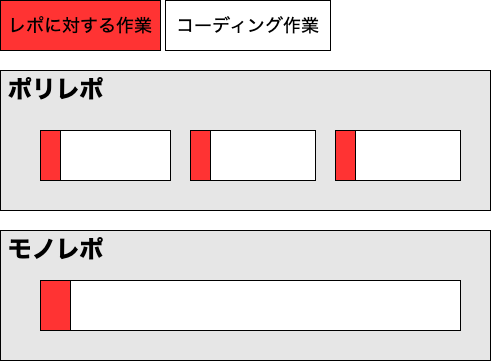
\includegraphics[height=150pt]{efficiency.png}
\end{frame}

\begin{frame}
    \frametitle{本質を探ろう --- 凝縮度と結合度}
    \begin{block}{}
        \centering
        \begin{tabular}{cc}
            \toprule
            メリット & デメリット \\
            \midrule
            作業効率 & 作業効率 \\
            \textcolor{red}{凝集度} & \textcolor{red}{結合度} \\
            \bottomrule
        \end{tabular}
    \end{block}
\end{frame}

\begin{frame}
    \frametitle{本質を探ろう --- 凝縮度と結合度}
    \only<2-3>{
        \onslide<2-3>{
            \begin{block}{凝集度}
                {\textit{単一\textcolor{red}{モジュール内}の要素間の関連性についての尺度。}}
            \end{block}
        }
        \onslide<3>{
            \begin{block}{結合度}
                {\textit{\textcolor{red}{モジュール間}の関連性についての尺度。}}
            \end{block}
        }
    }
    \only<4->{
        \begin{block}{凝集度}
            {\textit{単一\textcolor{red}{レポジトリ内}の要素間の関連性についての尺度。}}
        \end{block}
        \begin{block}{結合度}
            {\textit{\textcolor{red}{レポジトリ間}の関連性についての尺度。}}
        \end{block}
    }
    \onslide<3>{
        \vskip5mm
        \hspace*\fill{\small--- \href{https://www.ogis-ri.co.jp/otc/hiroba/technical/Cohesion_Coupling/Cohesion_Coupling.html}{オージス研}}
    }
\end{frame}

% \begin{frame}
%     \frametitle{異議あり!論点を掘り下げてみよう!}
%     \begin{itemize}
%         \item No overhead to create new projects --- 「PJ」 と 「レポ」を混同してない?
%         \item Shared code and visibility --- どうやってシェアするの?ライブラリ?直接参照?それ,モノレポじゃなくてもできるくない?
%         \item Atomic commits across projects --- 実は異議なし.それは本当にそう.だけど,誤解しちゃだめ (lockstep リリース)
%         \item One version of everything --- それ本当に良いことなのか?
%     \end{itemize}
% \end{frame}